\chapter*{Introduction}
\addcontentsline{toc}{chapter}{Introduction}

%surement qu'il faudrait mettre le classique de la réalisation de tte introduction: accroche , problématique, analyse du devellopement du plan

\section{Concevoir dans un champ social}
%Ouaouh! on a construit des robots pour aller sur la lune mais le mettre avec des humains c'est plus difficile

L’industrie, la technique et la recherche sont déjà investies par les robots. Mais quand les considérerons-nous comme des partenaires à part entière de notre vie ? C’est à cette question que tend à répondre ce projet de desserte robotisée.

C’est à l’origine dans le domaine de l’industrie, notamment automobile, que les robots se sont d’abord et le plus durablement installés. Pour ensuite se trouver dans les zones nucléaires, les terrains minés, l’espace ou les abysses marins à très forte pression. Et c’est ainsi que le robot a su se faire une place dans ces milieux dit « extrêmes ». Mais il n’est pas encore très bien adapté au secteur du service.

Faire entrer un robot chez soi reste pour beaucoup un grand pas à franchir. Il faut donc réussir à faire rentrer le robot dans notre société de façon subtile. Alors l’acceptation du robot comme un atout pour l’être humain, et non comme un danger, deviendra possible.

A travers la desserte robotisée, nous offrons au robot une place de soutiens au service lors de cocktail. On l’intègre donc à une place de partenaire pour l’homme. Et c’est ainsi qu’il prend une place dans le champ humain sans s’y imposer de façon brusque.


\section{Le context du cocktail}

Avant de définir le robot à construire, il faut découvrir le lieu dans lequel il va interagir. Nous allons donc présenter ce qu’est un cocktail, où il se déroule, les gens qu’on y retrouve, les ambiances et les interactions qui y sont commune.

\subsection{Où se déroule un cocktail}
%lister les lieux

%tous les lieux d'évènment
%Reception officiel et ou diplomatique
%Artistique
%Culturel
%Célébration (Mariage, remise de diplome, ventes...)
%les lieux d'interconnection de modalité de transport
%Inoguration
%espace grand
%Terrasse -> la merde en faisabilité
%Hotel, Galerie, Musée
%Jardin -> critique faisabilité impossibilité
%Gare
%Aeroport
%Salle de reception
%Restaurant
%Salle de bal

Un cocktail est un lieu de connexion entre les gens. C’est pourquoi il s’accorde avec les lieux d’interconnexion et d’évènementiel dans lequel les gens se retrouvent. Et ces lieux se déclinent entre les lieux dits de la « haute société » et ceux plus populaires. Leurs tailles se déclinent par rapport aux nombres de personnes s’y retrouvant, d’une vingtaine dans $25m^2$ à un peu plus de 200 dans une superficie proportionnellement équivalente.

Les lieux d’interconnexion sont des lieux qui sont placé de telle sorte qu’il y a de grande chance d’y amener le plus de gens sans qu’ils n’aient à se déplacer vers un lieu précis. Par exemple une gare ou aéroport voir un lieu courant où passe tous les éléments d’une compagnie. On n’y retrouve pas forcement de logique évènementiel mais ces lieux peuvent se lier à un évènement tel qu’une inauguration.

Les lieux évènementiel, comme les musées, les hôtels ou les galeries, n’ont pas la même logique spatial que les lieux d’interconnections.  C’est lieux peuvent avoir une logique artistique ou culturel mais l’évènement peut aussi être une réception officiel ou diplomatique. C’est un cocktail qui est souvent lié à une célébration comme un mariage ou une remise de diplômes.

Dans ces lieux, on y retrouve les castes de société qui y sont définit. C’est groupes sociétales sont définis par le lieu lui-même et l’évènement. Par exemple « le bal des débutantes » ne réunira par le même type de groupe sociétal que les artistes d’une galerie d’art.


\subsection{Qui sont les acteurs du cocktail}
%lister les personnes

%Prestataire* / Maitre d'Hotel / Traiteur.
%Serveurs
%Nettoyeurs
%Invités
%Organisateur (pas forcement le prop)
%Le propriétaire de la salle

Le cocktail n’est pas seulement un lieu où se retrouve convive et serveur. C’est avant tout une salle offerte par son propriétaire. Cette personne peut tout aussi bien être le prestataire tel le maître d’hôtel, l’organisateur ou encore un invité.

Ensuite il y a l’organisateur, il invite les convives et est le prestataire ou en engage un.

Le prestataire fournit au cocktail toute sa partie matérielle. C’est-à-dire les apéritifs et l’alcool ainsi que le service. Dans le service nous retrouvons les serveurs. Qui sont donc engagés par l’organisateur et qui servent les invités.

Un cocktail sans invité n’aurait aucune logique, ils sont les personnages les plus importantes du cocktail, servis par les serveurs et invité par l’organisateur.

Et après le cocktail, il faut nettoyer la salle. . Il y a donc les nettoyeurs qui font partie du cocktail même si on ne les remarques pas.

\subsection{Les ambiances d'un cocktail}
%lister les qualités

%Tendu
%Affaires - diplomatique
%Classe -> ambiance feutré bien habillé.

%Détendu
%Galeire, vernissage
%Artistique -> Moins strict

%adapté à ces deux niveau visuel.

Les ambiances du cocktail sont un élément en grande partie régis par les convives. Ils sont, par leurs attitudes et leur vision des autres convives, l’atmosphère des ambiances. 
Il y a des cocktails avec des ambiances plus tendu que d’autres ce qui est souvent liée à des règles de conduites plus stricts. C’est règles sont remarqué tout d’abords par une tenue, l’éducation et la classe des smokings n’est pas la même.  Ensuite elle se démarque par la logique de retrouvaille. 

Lorsqu’un cocktail est organisé pour un vernissage ou une avant-première, nous sommes dans un milieu artistique. On retrouve lors du cocktail des gens venu pour acheter, d’autres pour voir les œuvres et pour parler aux artistes.

Lorsqu’un cocktail d’affaire ou à but diplomatique est organisé, nous sommes dans une ambiance plus feutré.  Les personnes dans ce cocktail cherchent à se mettre en relation pour préparer des affaires futures.

Le but du serveur face à ces deux types de convives n’est pas de faire partie de leurs groupes mais de les servir. Il aura donc des relations de service pour rendre plus agréable l’évènement. C’est à dire qu’il est là pour faire gagner du temps aux invités en leurs amenant leurs amuse-bouches et leurs verres d’alcool et de pouvoir les indiquer sur les diverses éléments du cocktail. Il est aussi un léger lien de communication pour lier deux groupes de personnes entre elles ou faire passer un message de façon subtile comme un appel. 


\subsection{Les complexités des niveaux d'interactions dans le cocktail}
%lister les "`enjeux"' qui amènent les intéractions

Comme expliqué dans les parties précédentes, il y a 6 personnes, distincts ou non, qui participent au cocktail. Le propriétaire de la salle, l’organisateur, le prestataire, les serveurs, les invités et les nettoyeurs.

Le propriétaire voit avec l’organisateur pour la réalisation du cocktail. L’organisateur embauche un prestataire. Le prestataire réalise le cocktail avec ses serveurs. Les serveurs servent les invités. Les invités discutent entre eux. Le prestataire demande de nettoyer aux nettoyeurs.

Tout se retrouve donc à travers un graphique.

\begin{figure}[h]
\begin{center}
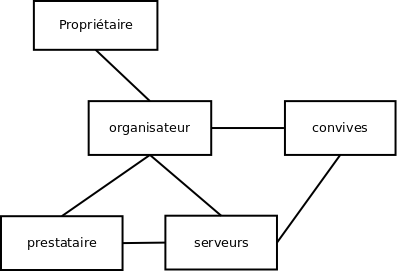
\includegraphics[scale=0.55]{Images/interaction_cocktail.png}
\caption{Diagramme des interactions d'un cocktail}
\label{Diagramme des interactions d'un cocktail}
\end{center}
\end{figure}

%Pour chaque acteur il faut définir leur relation.

% Propriétaire -> Orga -> prest -> Netoyaire et Serveur(boucle) -> convives (boucles)
